\uuid{Opt102}
\titre{Fonction deux variables}
\theme{optimisation}
\auteur{Jean-François Culus}
\organisation{AMSCC}
\contenu{

\texte{Déterminer les extrémums locaux des applications suivantes définies sur $\R^2$:


\begin{enumerate}
\item 
\question{$f(x,y)= 4x + 2y - x^2- y^2 - 2x^3$}
\reponse{
Les dérivées partielles de \( f(x, y) \) sont :

\[
\frac{\partial f}{\partial x} = 4-2x-6x^2
\]

\[
\frac{\partial f}{\partial y} = 2-2y
\]

Ainsi, recherchons les points critiques, c'est-à-dire vérifiant $\frac{\partial f}{\partial x} (x,y)=\frac{\partial f}{\partial y} (x;y)=0$.
\\ Nous obtenons alors que $6x^2+2x-4=0$ soit $3x^2+x-2=0$. En calculant le discriminant, nous obtenons que 
$\Delta=25$, donc que les racines de cette équation d'ordre $2$ sont $x=-1$ et $x=2/3$.
La seconde condition portant sur $y$ donne $y=1$: ainsi, il y a deux points critiques, 
$A:(-1;1)$ et $B:(2/3;1)$. 
\\ Nous savons que si $f$ admet un extremum local, comme $f$ est de classe $\mathcal{C}^1$ sur $\R^2$ (c'est une fonction polynomiale en $(x,y)$), celui ci est nécessairement un point critique. 

Pour déterminer la nature du point critique, calculons la matrice Hessienne: 
\[
H(x,y) = \begin{bmatrix}
\frac{\partial^2 f}{\partial x^2} & \frac{\partial^2 f}{\partial x \partial y} \\
\frac{\partial^2 f}{\partial y \partial x} & \frac{\partial^2 f}{\partial y^2}
\end{bmatrix}
=
\begin{bmatrix}
-2-12x & 0 \\
0 & -2
\end{bmatrix}
\]

Pour le point $A$, nous obtenons alors $H(-1;1)= \begin{pmatrix} 10 & 0 \\ 0 & -2\end{pmatrix}$ de déterminant 
$-20$. Ainsi, le déterminant étant négatif, $A$ est un point selle. 

Pour le point $B$, nous obtenons 
$H(2/3;1) = \begin{pmatrix} -10 & 0 \\ 0 & -2\end{pmatrix}$, de déterminant $20>0$ donc cette fonction admet un extrémum en $B$.  Comme $\frac{\partial^2 f}{\partial x^2}<0$, nous en déduisons que c'est un maximum. 


Ainsi, $f$ admet un maximum local en $B$.

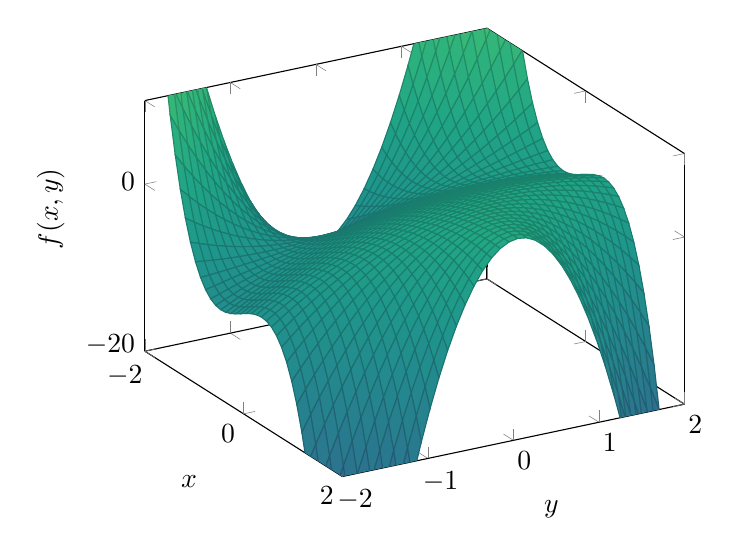
\begin{tikzpicture}
    \begin{axis}[
        view={60}{30},        % Angle de vue
        colormap/viridis,     % Colormap pour les couleurs
        domain=-2:2,          % Domaine des variables x et y
        samples=40,           % Nombre d'échantillons
        xlabel=$x$,           % Étiquette pour l'axe x
        ylabel=$y$,           % Étiquette pour l'axe y
        zlabel={$f(x,y)$},    % Étiquette pour l'axe z
        zmax=10,              % Limite maximale de l'axe z
        zmin=-20              % Limite minimale de l'axe z
    ]
    \addplot3[
        surf,                 % Style de tracé en surface
    ]
    {4*x + 2*y - x^2 - y^2 - 2*x^3*y^2};    % Fonction à tracer
    \end{axis}
\end{tikzpicture}

}

\item \question{$g(x,y)=xy+x^3y^2$}
\reponse{
Les dérivées partielles de \( g(x, y) \) sont :

\[
\frac{\partial f}{\partial x} = y+3x^2y^2 \]
\[
\frac{\partial g}{\partial y} = x+2x^3y \]

Ainsi, recherchons les points critiques, c'est-à-dire vérifiant $\frac{\partial g}{\partial x} (x,y)=\frac{\partial g}{\partial y} (x;y)=0$.
\\ Nous obtenons alors que $y(1+3x^2y)=0$ et $x(1+2x^2y^2)=0$. 

Raisonnons alors par disjonction des cas: si $y=0$ (1ere équation), alors nécessairement $x=0$ (seconde équation). 
\\ Si $1+3x^2y=0$, alors si $x=0$ ce qui est absurde ($1=0$), soit c'est $1+2x^2y=0$.
Cela conduit alors à $x^2y=0$, d'où $x=0$ ou $y=0$, ce qui est ici absurde (hypothèse $1+3x^2y=0$).

Nous en déduisons donc que l'unique point critique de la fonction $g$ est le point $(0;0)$.

Reste à étudier si ce point est un extrémum local ou non.  
Pour ce faire, calculons la Hessienne de cette fonction. Nous obtenons:

\[
H(x,y) = \begin{bmatrix}
\frac{\partial^2 g}{\partial x^2} & \frac{\partial^2 g}{\partial x \partial y} \\
\frac{\partial^2 g}{\partial y \partial x} & \frac{\partial^2 g}{\partial y^2}
\end{bmatrix}
=
\begin{bmatrix}
6xy^2 & 1+6x^2y \\
1+6xy & 2x^3  
\end{bmatrix}
\]

Ainsi, l'évaluation de la Hessienne au point critique $(0,0)$ donne $H(0,0)=\begin{pmatrix} 0  & 1\\ 1&0\end{pmatrix}$. Son déterminant est négatif, d'où $(0,0)$ est un point selle. 
La fonction $g$ n'admet donc ni minimum ni maximum local. 

Pour le point $A$, nous obtenons alors $H(-1;1)= \begin{pmatrix} 10 & 0 \\ 0 & -2\end{pmatrix}$ de déterminant 
$-20$. Ainsi, le déterminant étant négatif, $A$ est un point selle. 

Pour le point $B$, nous obtenons 
$H(2/3;1) = \begin{pmatrix} -10 & 0 \\ 0 & -2\end{pmatrix}$, de déterminant $20>0$ donc cette fonction admet un extrémum en $B$.  Comme $\frac{\partial^2 f}{\partial x^2}<0$, nous en déduisons que c'est un maximum. 


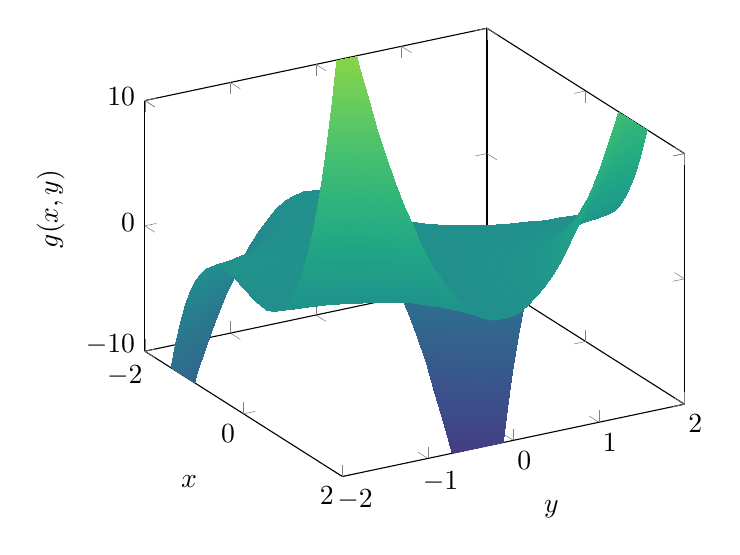
\begin{tikzpicture}
    \begin{axis}[
        view={60}{30},         % Angle de vue (azimuth, elevation)
        colormap/viridis,      % Colormap pour les couleurs
        domain=-2:2,           % Domaine des variables x et y
        samples=40,            % Nombre d'échantillons pour chaque variable
        xlabel=$x$,            % Étiquette pour l'axe x
        ylabel=$y$,            % Étiquette pour l'axe y
        zlabel={$g(x,y)$},     % Étiquette pour l'axe z
        zmax=10,               % Limite maximale de l'axe z
        zmin=-10               % Limite minimale de l'axe z
    ]
    \addplot3[
        surf,                  % Style de tracé en surface
        shader=interp,         % Interpolation des couleurs pour lisser la surface
    ]
    {x*y + x^3*y^2};           % Fonction à tracer
    \end{axis}
\end{tikzpicture}

}
\end{enumerate} } 
} 